\documentclass[0-thesis.tex]{subfiles}

\begin{document}
The previous sections proposed the update architecture of the thesis, its key components,
and security considerations such as identity and access control. This section will discuss
a prototype implementation of the architecture as well as a manifest generator. 

\subsection{Prototype Design}
\label{ssec:prototype-design}
% TODO: Cite the repository (consider branches)
The prototype is developed as a means of evaluating the efficiency of the transport during
an update procedure. It consists of an update server and a client (device). The prototype
is using a pull model where the device initiates the update procedure. The notion of an
operator is cut out as it will not be used in a real deployment, as such there is only the
update server and client.

Contiki-NG, introduced in Section~\ref{sec:contiki-ng}, is the operating system of choice
for both the client and server. It is an operating system suitable for constrained devices
such as those of wireless sensor networks. Contiki-NG comes with a network stack featuring
CoAP(s) and DTLS which are the target protocols for the prototype. The reason for
implementing the update server prototype in Contiki-NG is as a proof of concept that a
more capable IoT device in a network could act as an update server. Of course, storage for
the firmware images hosted on the server must be accomodated for, a real deployment might
opt to use the Coffee filesystem together with Contiki-NG \parencite{coffee}. The server
prototype of this thesis runs as a native Contiki-NG process on a host computer (thus
using the host computers' filesystem), while the client was developed natively then ported
to a Firefly board. The implementation is found in the \texttt{examples/suitup} directory
of the project repository \parencite{suitup}. % TODO: Port not yet done, have no hardware

The interactions of the client and server are simplistic and the client has no other
behaviour than to initialize and complete the update procedure. As shown in
Figure~\ref{fig:client-server-interaction}, the interaction starts with a POST request
from the client to the registration endpoint of the server. The registration is sent as a
confirmable CoAP packet and is thus acknowledged. Afterwards, the client sends a GET
request for a manifest. The idea is that the endpoint \texttt{update/manifest} is a well
known endpoint just like \texttt{update/register} and all devices in the network register
and poll for manifests at these endpoints. Upon a request to \texttt{update/manifest} it
is up to the server to decide whether there is a suitable manifest or not, the decision
making is offloaded from the device. The prototype only makes use of one manifest thus
such logic is not implemented, but in real deployments the \texttt{update/manifest}
resource would handle that (using the information from the devices' profile).

% TODO: Mention keys and certs for DTLS and COSE once it is figured out

\begin{figure}
    \caption{The interactions of client and server during an update procedure.}
    \label{fig:client-server-interaction}
    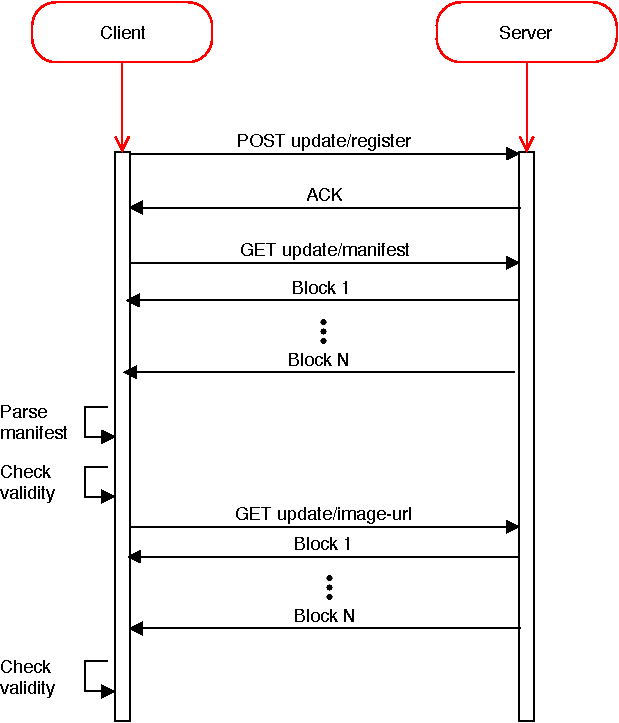
\includegraphics{images/client-server-sequence.pdf}
\end{figure}

If a suitable manifest is found, it is then transferred back to the client. As most
manifests will be too large for a single CoAP message, the server makes use of the block
option in CoAP. The manifest is split in chunks that are sent one by one. The client
receives these chunks and reassembles the manifest as it is received. After the manifest
in its entirety has been transferred, the client parses the manifest and checks its
validity by comparing vendor and class IDs. As described in
Section~\ref{ssec:manifest-format} there can be more preconditions requiring more checks,
again this is deployment specific. 

If the client deems the manifest to be valid it requests the update image from the URL
specified in the manifest. The endpoint is now specific for this particular class of
device and version and is not known in advance, it must be in the manifest. The image,
also too large for a single CoAP message, is transferred in blocks. When the client has
received the image, it calculates the SHA-256 hash of it, comparing it to the hash
contained in the manifest. This concludes the transfer of an update.

\subsection{Manifest Implementation}
\label{ssec:manifest-implementation}
As manifests contain certain information difficult for humans to provide such as
monotonically increasing sequence numbers and digests, a manifest generator was created to
help test the prototype \parencite{manifest-generator}. It is a Python script which
accepts information about vendor and class namespace, version, image, and associated URL
to generate, format, and output a manifest both in JSON and CBOR. The outputted manifest
follows the format specified in Section~\ref{ssec:manifest-format} and features all
required fields although many left blank. It is a bare-bones manifest containing only the
required information for a singular, monolithic update. There are no dependencies or
options. 

The manifest is a JSON map featuring the required elements shown in
Figure~\ref{fig:manifest-format}. The elements are in the same order as in the figure but
the names of the fields have been substituted for integers in order to save space.
Table~\ref{tab:manifest-substitution} shows this mapping. Nested structures such as
preconditions are described as an array of maps, where each map in the array consitutes
one precondition. The keys for these maps are also mapped to integers as in the main
manifest structure, resetting the counter for each nested structure. The mapping of keys
in nested structures is shown in Table~\ref{tab:nested-substitution}. Dependencies,
precursor image lists, URL/digest pairs, and options are described in the same way even
though the example manifest leaves most of these fields empty. The example manifest used
can be found in Appendix X. 

\begin{longtable}[]{@{}ll@{}}
    \caption{Mapping manifest elements to integers as keys in the JSON manifest.}
    \label{tab:manifest-substitution}\\
    \toprule
    Element name & Integer\tabularnewline
    \midrule
    \endhead
    versionID & 0\tabularnewline
    sequenceNumber & 1\tabularnewline
    preConditions & 2\tabularnewline
    postConditions & 3\tabularnewline
    contentKeyMethod & 4\tabularnewline
    payloadInfo & 5\tabularnewline
    precursorImage & 6\tabularnewline
    dependencies & 7\tabularnewline
    options & 8\tabularnewline
    \bottomrule
\end{longtable}

\begin{longtable}[]{@{}ll@{}}
    \caption{Mapping elements in nested structures to integers.}
    \label{tab:nested-substitution}\\
    \toprule
    Element name (corresponding structure) & Integer\tabularnewline
    \midrule
    \endhead
    type (conditions and options) & 0\tabularnewline
    value (conditions and options) & 1\tabularnewline
    \bottomrule
    URL (URL/digest pair) & 0\tabularnewline
    digest (URL/digest pair) & 1\tabularnewline
    \bottomrule
    format (payload info) & 0\tabularnewline
    size (payload info) & 1\tabularnewline
    storage (payload info) & 2\tabularnewline
    URL/digest pair (payload info) & 3\tabularnewline
    \bottomrule
\end{longtable}

In the client code, the manifest is received as a string, still formatted as JSON. In
order to parse it, structs resembling the format of the manifest were created. Nested
elements such as preconditions are implemented as linked lists, where each precondition
contains a type, a value, and a pointer to the next. The manifest structure contains a
pointer to the first precondition, from which the entire set of preconditions can be
retrieved. The set of structs and their relations are as in
Figure~\ref{fig:manifest-format}, where conditions, URL/digest pairs, and options are
implemented in a linked list way. This kind of structuring is extensible, allowing
implementors to easily add new conditions or options as well as specify an arbitrary
amount of dependencies, precursors, and mirrors of images.
    

% TODO: Include example manifest in appendix.

\end{document}